
\chapter{Solution methodology} \label{chap:methodology}

\bt

\section{Method 1}

\bt

\section{Method 2}

\bt 

\section{Method 3}

Some nice matrices...

\begin{equation}
	A = \begin{bmatrix}
		1 &    &    &    &    &    &    & \\
		1 & -2 &  1 &    &    &    &    & \\
		  &  1 & -2 &  1 &    &    &    & \\
		  &    &  1 & -2 &  1 &    &    & \\
		  &    &    &  1 & -2 &  1 &    & \\
		  &    &    &    &  1 & -2 &  1 & \\
		  &    &    &    &    &    &  1 & \\
	\end{bmatrix}
	\hspace{1cm}
	B = \begin{bmatrix}
		0 \\
		4 \\
		4 \\
		4 \\
		4 \\
		4 \\
		0
	\end{bmatrix}
\end{equation}

Some nice diagrams...

\newcommand{\cv}[1]{ % column vector
	$\begin{bmatrix} #1 \end{bmatrix}$
}
\newcommand{\Cv}[1]{ { \cv{#1} } } % shortcut for tree leaves
\newcommand{\elim} { $\xrightarrow{E}$ }
\newcommand{\merge} { $\xrightarrow{M}$ }
\newcommand{\xtract} { $\xrightarrow{X}$ }

\begin{figure}[H]
	\centering
	\caption{Elimination tree for multifrontal solver}
	\label{fig:mfs-elim-tree}
	\begin{forest}
		for tree = {
			draw,
			edge={<-, line width=2pt},
			minimum height=2cm,
			anchor=north,
			align=center,
			child anchor=north
		},
		[ { \merge \cv{x_1 \\ x_5 \\ x_7} \elim \cv{x_1 \\ x_7 } }
			[ { \merge \cv{x_1 \\ x_3 \\ x_5} \elim \cv{x_1 \\ x_5} }
				[ { \merge \cv{x_1 \\ x_2 \\ x_3} \elim \cv{x_1 \\ x_3} }
					[ \Cv{x_1 \\ x_2} ]
					[ \Cv{x_2 \\ x_3} ]
				]
				[ { \merge \cv{x_3 \\ x_4 \\ x_5} \elim \cv{x_3 \\ x_5} }
					[ \Cv{x_3 \\ x_4} ]
					[ \Cv{x_4 \\ x_5} ]
				]
			]
			[ { \merge \cv{x_5 \\ x_6 \\ x_7} \elim \cv{x_5 \\ x_7} }
				[ \Cv{x_5 \\ x_6} ]
				[ \Cv{x_6 \\ x_7} ]
			]
		]
	\end{forest}
\end{figure}

\pagebreak

Some nice algorithms...

\newcommand{\U}{\mathcal{U}}

\begin{algorithm}
\caption{One iteration of the double-grid algorithm}
\label{alg:two-grid}

\begin{algorithmic}

	\State Compute the solution $\U^C$ on the coarse mesh
	\State Split each element of the coarse mesh, thus obtaining the fine mesh
	\State Compute the solution $\U^F$ on the fine mesh

	\For{\textbf{each} coarse mesh element $\eps_i$}
		\LineComment{$\rho_i$ is the relative error}
		\State $ \rho_i \gets \left|
				\frac {
					\U^F_i - \U^C_i
				} {
					\U^F_i
				}
			\right| $
	\EndFor

	\State $\rho_{max} \gets$ $max_i(\rho_i)$

	\For{\textbf{each} element $\eps_i$}
		\If {$ \rho_i > \tau \cdot \rho_{max} $}
			\State adapt the $\eps_i$ element (split into two halves)
		\EndIf
	\EndFor

\end{algorithmic}
\end{algorithm}

\pagebreak

Some nice figures...

\begin{figure}[H]
	\centering

	\caption[Double-grid h-adaptation strategy, steps 1-2] {
		Steps 1-5 of the double-grid h-adaptation strategy, quadratic B-splines
	}
	\label{fig:h-adapt-two-grid}

	\begin{subfigure}[h]{1.0\textwidth}
		\centering
		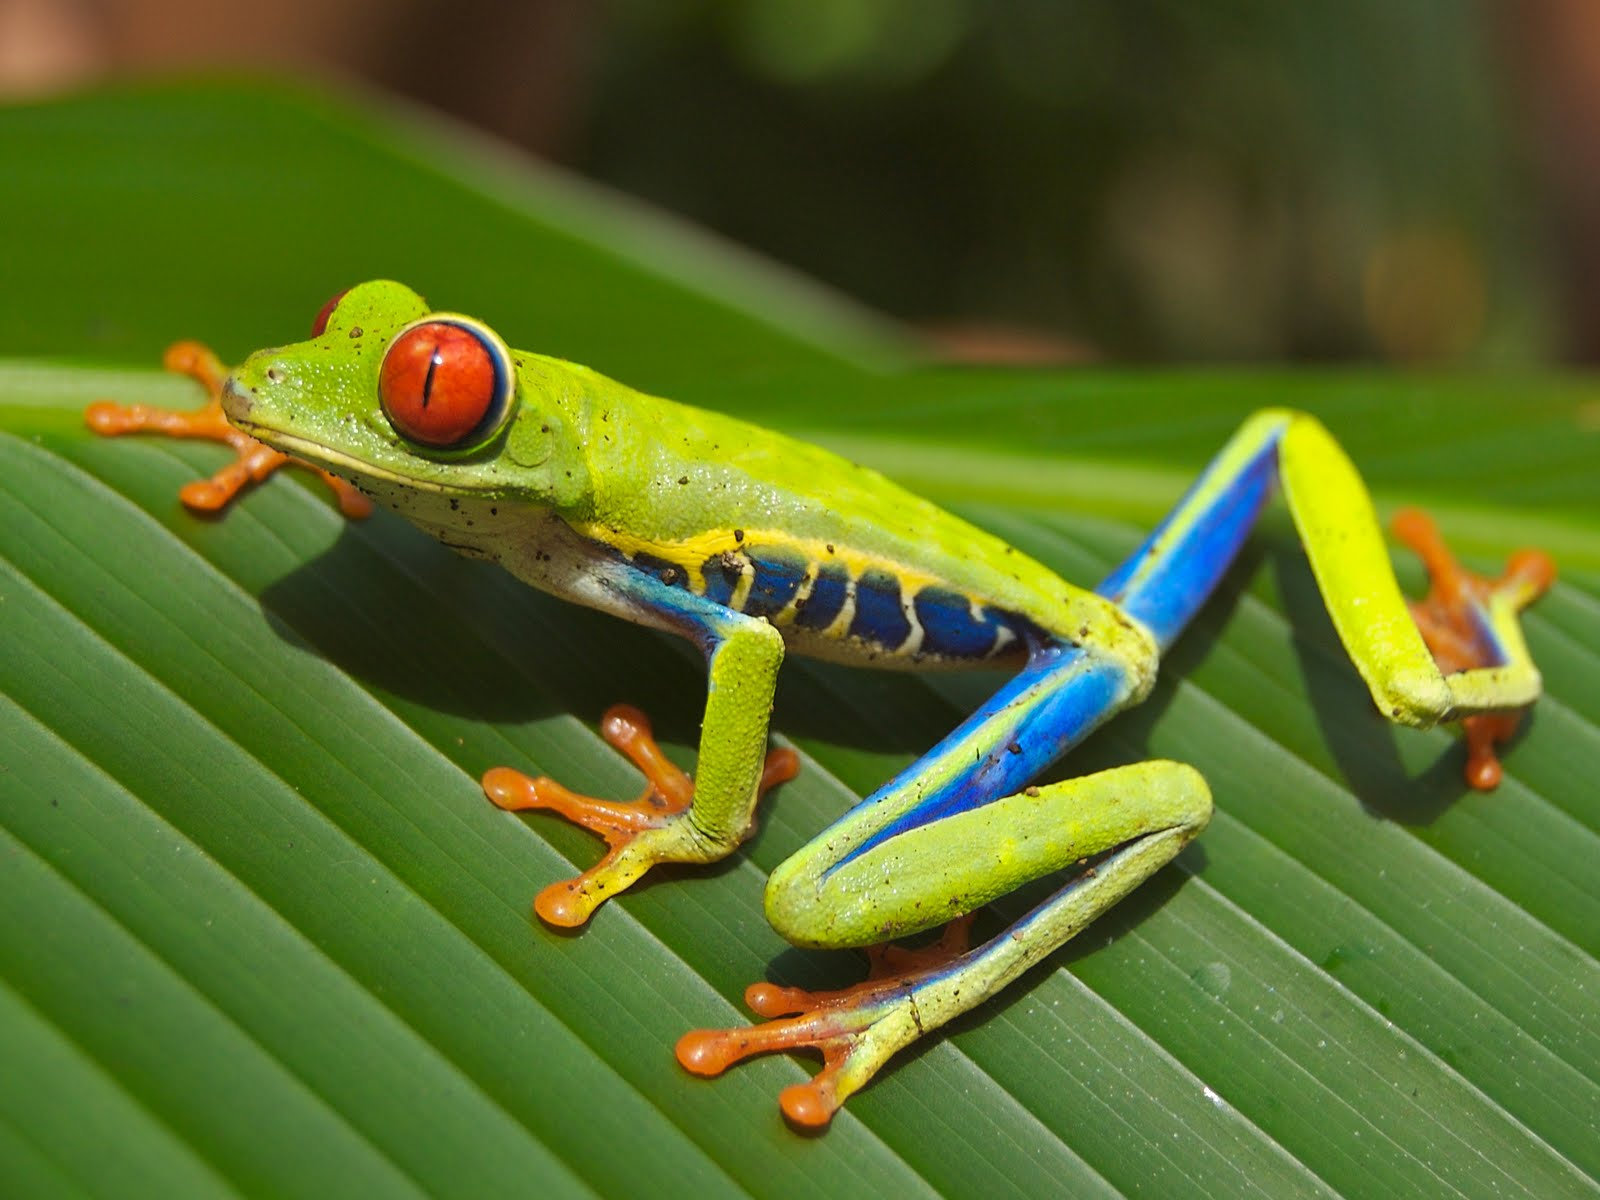
\includegraphics[scale=0.2]{frog.jpg}
		\caption{
			Step 1.
			A solution is delivered on coarse (4 elements) and fine grid (8 elements).
			Red line marks the coarse-grid solution, green line --- the fine-grid solution and black line --- the exact (analytic) solution.
		}
		\label{fig:h-adapt-two-grid-1}
	\end{subfigure}

	\begin{subfigure}[h]{1.0\textwidth}
		\centering
		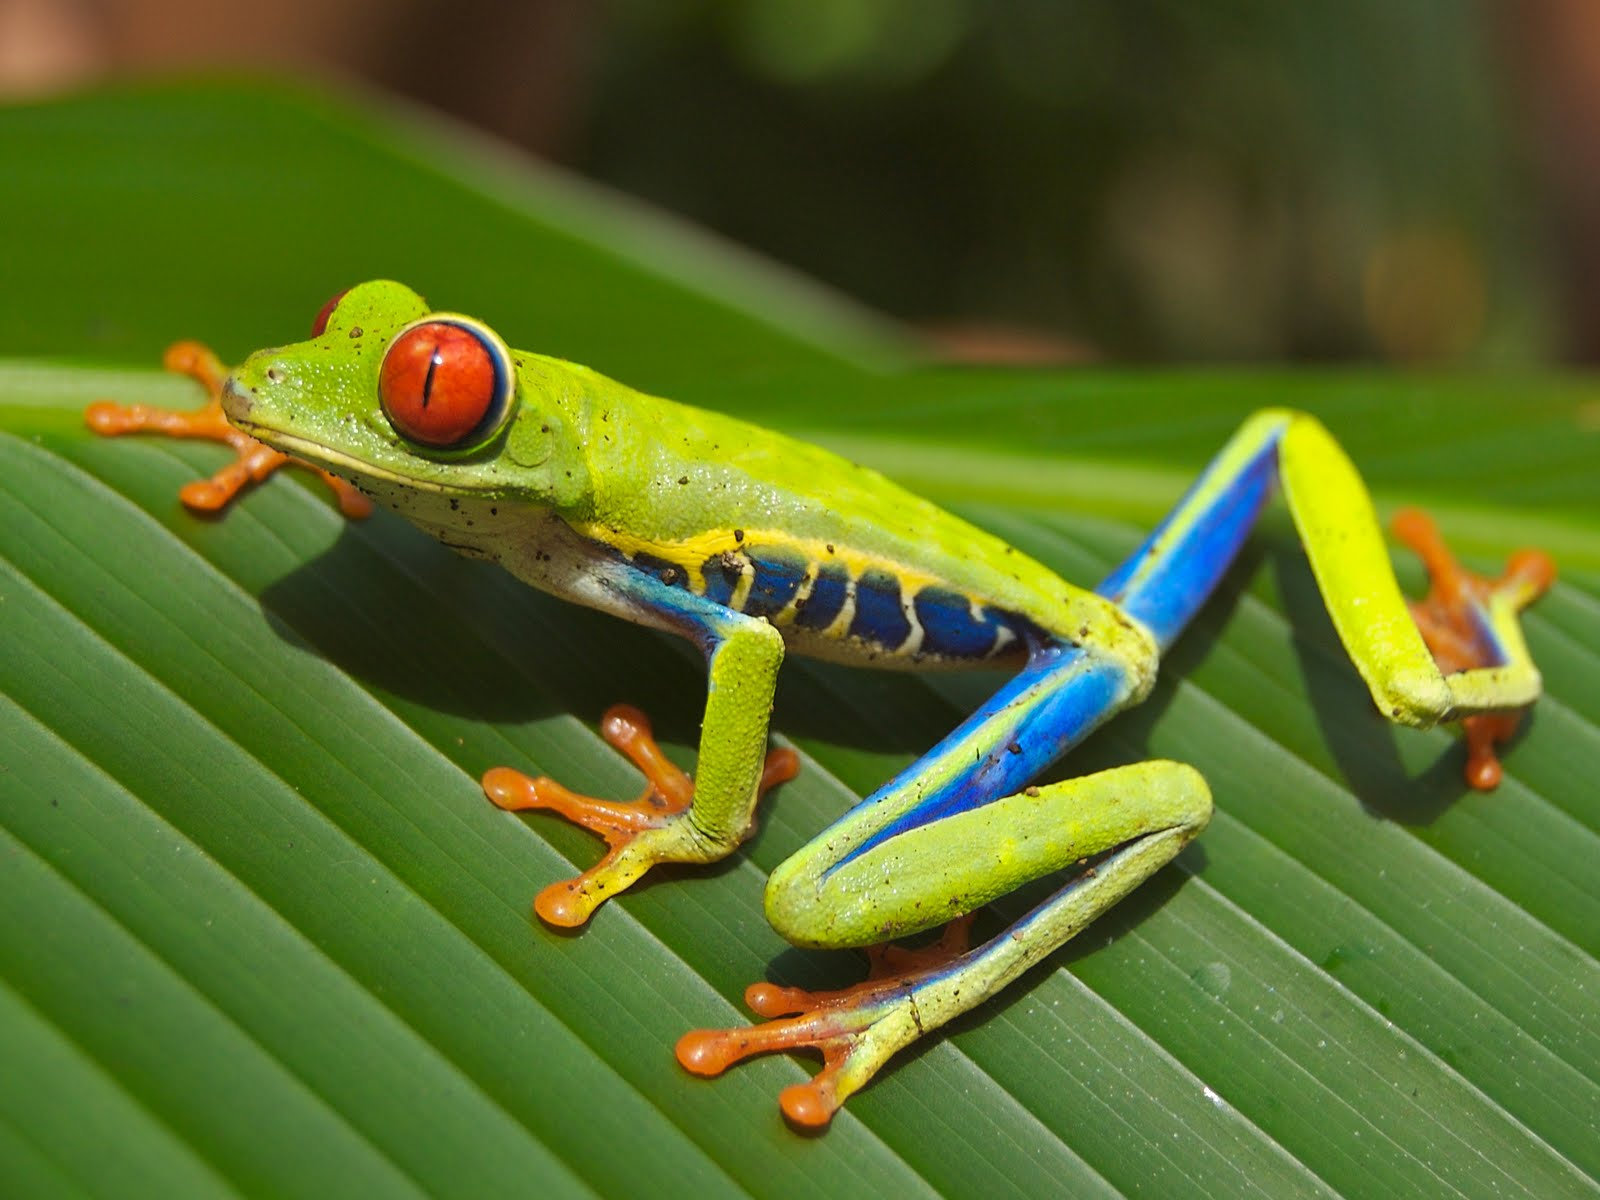
\includegraphics[scale=0.2]{frog.jpg}
		\caption{
			Step 2.
			Since the maximal error multiplied by $\tau$ (here set to 20\%) were lower than the error on any element,
			the algorithm halved all four elements after step 1.
		}
		\label{fig:h-adapt-two-grid-2}
	\end{subfigure}
\end{figure}


\begin{figure}[H]
	\ContinuedFloat % continue from previous page
	\caption[Double-grid h-adaptation strategy, steps 3-4]{} % for subcaption package to ensure proper numbering

	\begin{subfigure}[h]{1.0\textwidth}
		\centering
		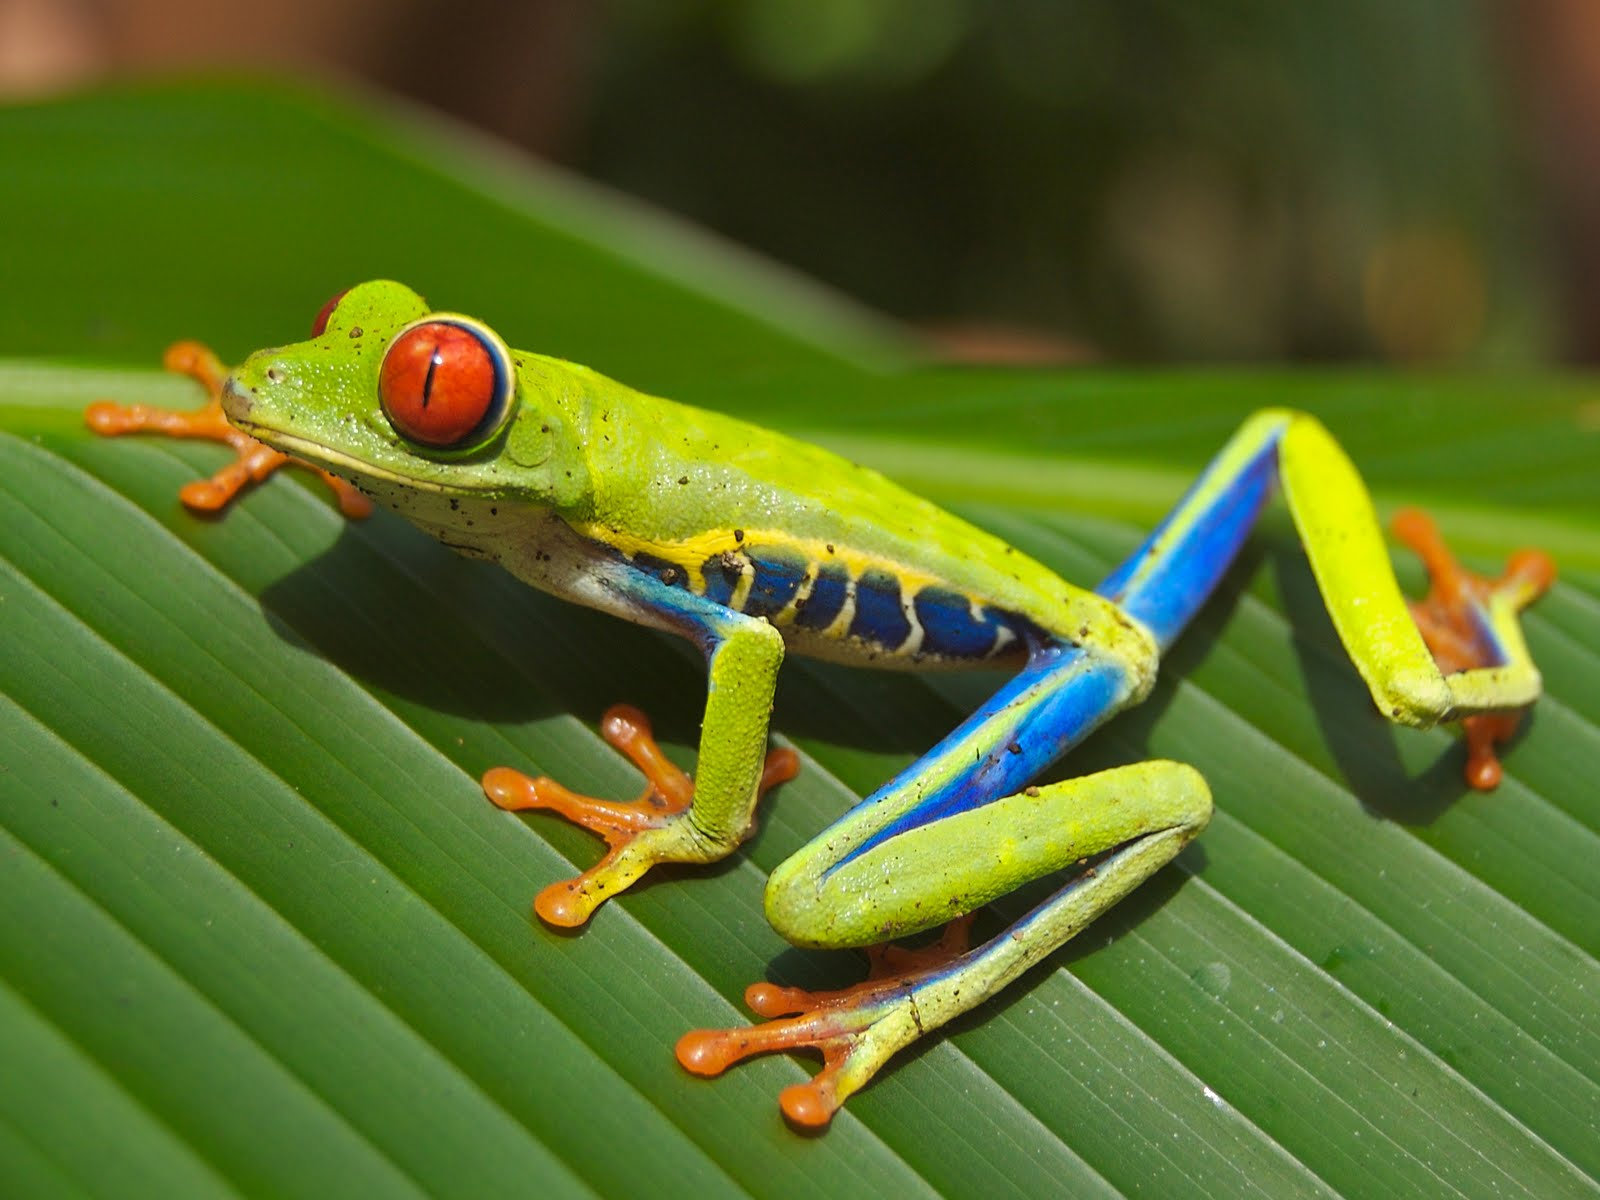
\includegraphics[scale=0.2]{frog.jpg}
		\caption{
			Step 3.
			The extreme left and right elements did not get refined after the step 2.
		}
		\label{fig:h-adapt-two-grid-3}
	\end{subfigure}

	\begin{subfigure}[h]{1.0\textwidth}
		\centering
		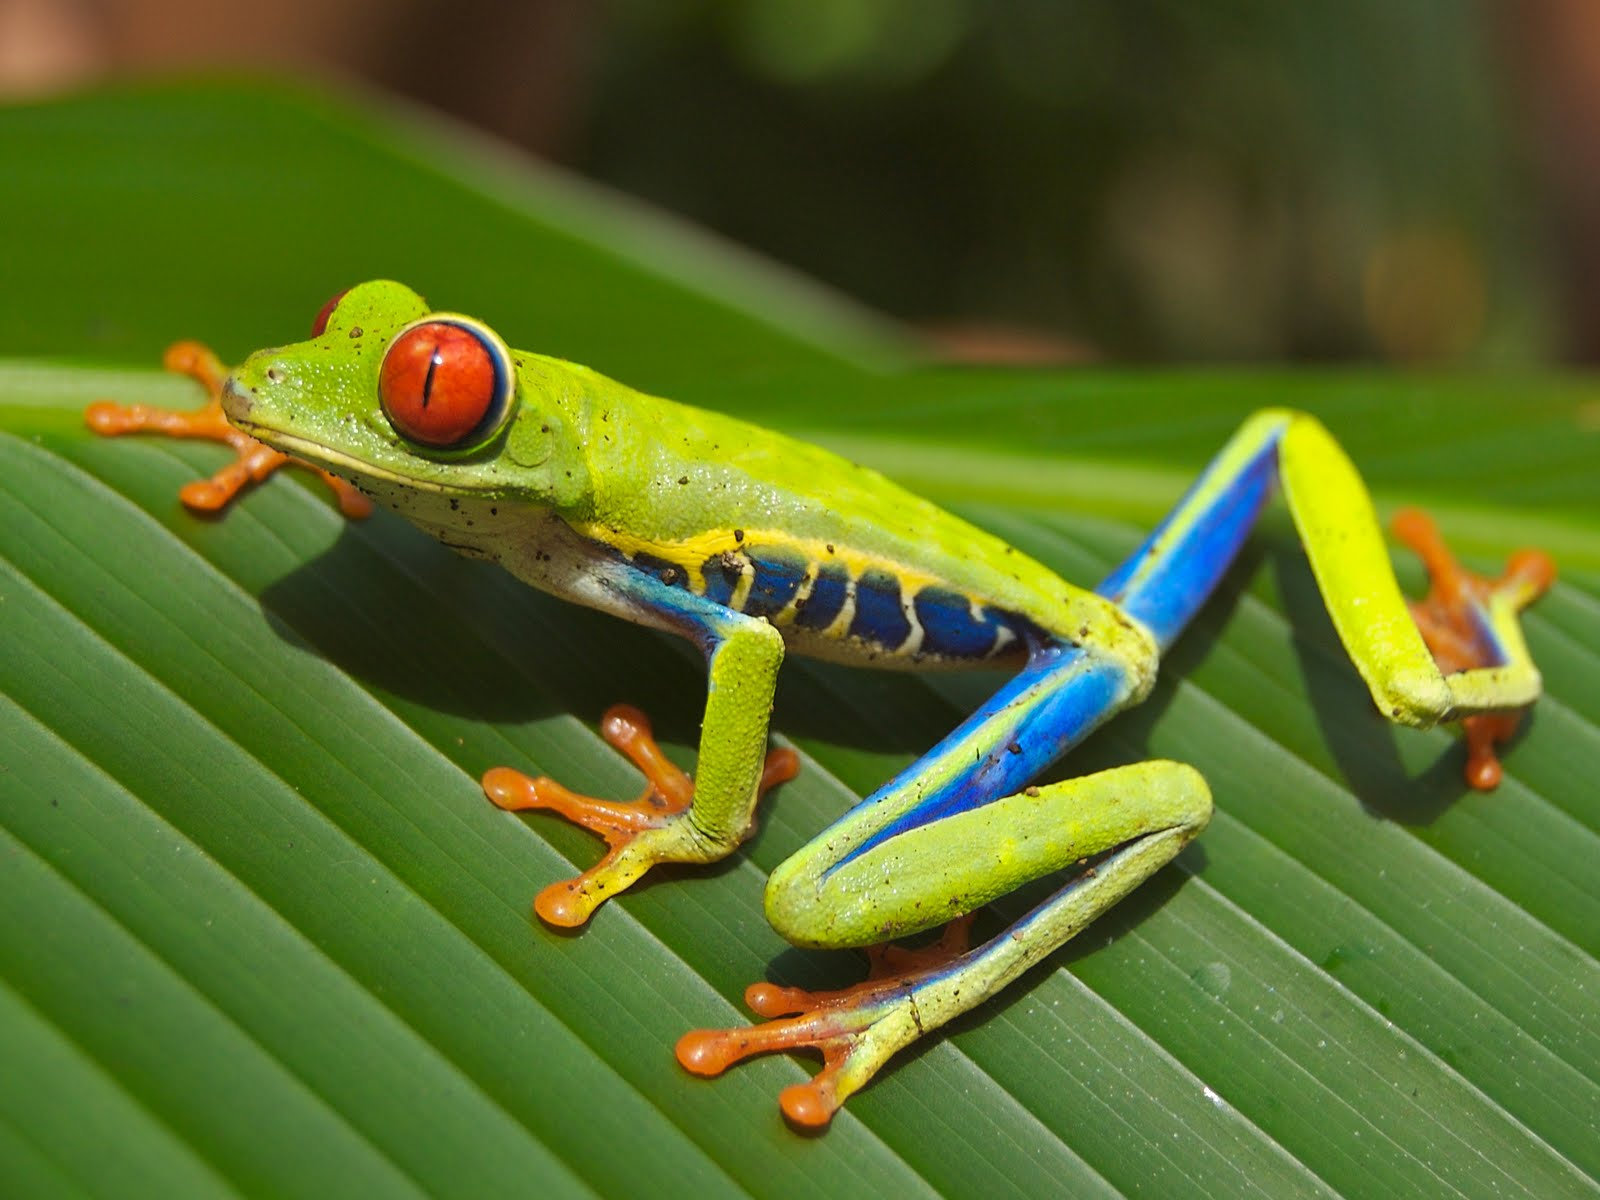
\includegraphics[scale=0.2]{frog.jpg}
		\caption{
			Step 4
		}
		\label{fig:h-adapt-two-grid-4}
	\end{subfigure}
\end{figure}


